% % Appendix Template

% \chapter{Acknowledgements} % Main appendix title

% \label{Ack} % Change X to a consecutive letter; for referencing this appendix elsewhere, use \ref{AppendixX}

% \lhead{\emph{Acknowledgements}} % Change X to a consecutive letter; this is for the header on each page - perhaps a shortened title
% % 
% % \addtocontents{toc}{} % Add a gap in the Contents, for aesthetics

% \addtotoc{Acknowledgements} % Add the "Abstract" page entry to the Contents 
\addtocontents{toc}{} % Add a gap in the Contents, for aesthetics
\thispagestyle{empty}
\acknowledgements{

I thank my parents for always motivating me. I would also like to express gratitude to my guide: Prof. Debasattam for introducing me to this fascinating topic. Most of the content here is inspired by \cite{vanwaarde2023informativity, 9781279, 9551767, 10383531, brunton2021modern}, many statements are directly taken from here and my explanations are based on my understanding from these papers. And, lastly thanks to you, reader, I have worked hard in making this thesis, in the hope that this work helps you in some way.
\begin{figure}[H]
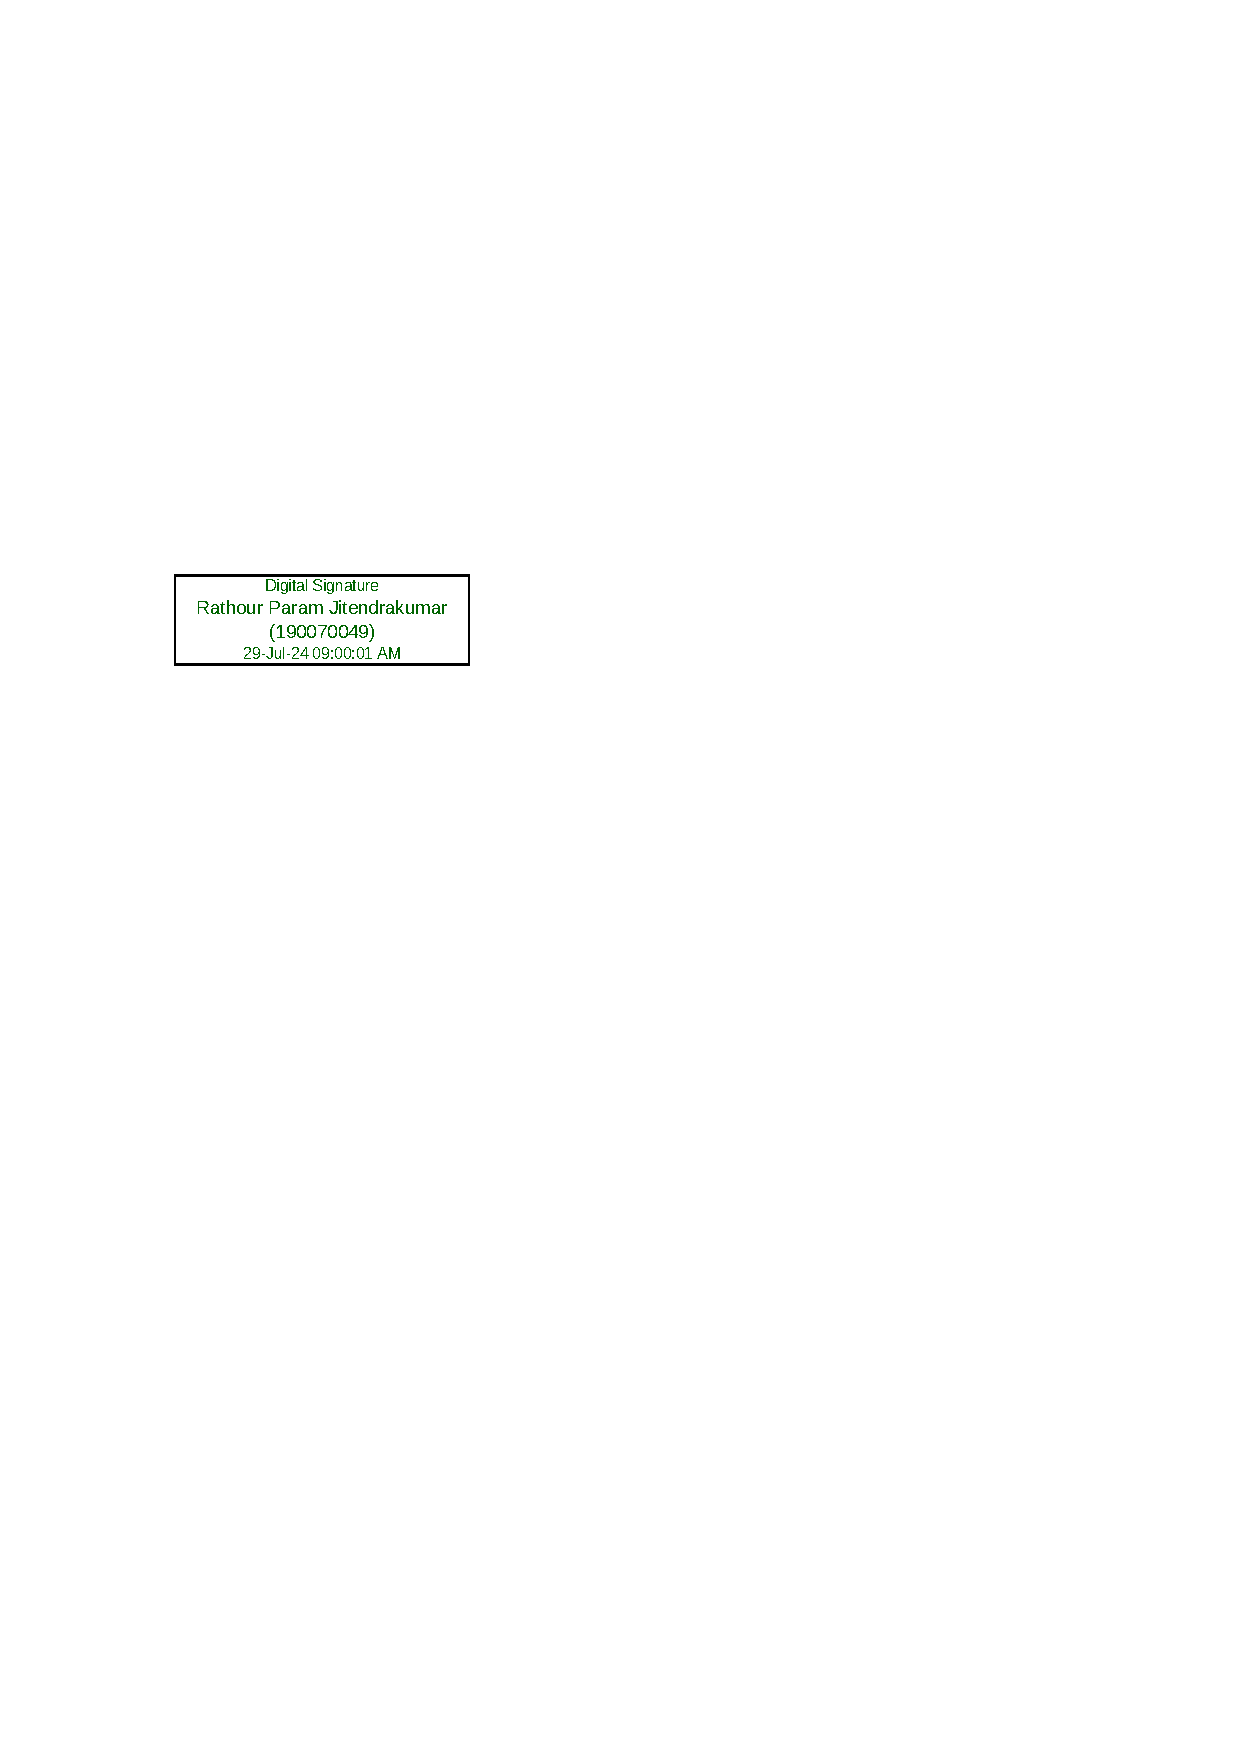
\includegraphics{ACK.pdf}
\end{figure}
\vspace{-3em}
\begin{flushleft}
    \textbf{\authornames}
\end{flushleft}
}
\begin{textblock*}{\textwidth}(3cm,31.65cm) % Adjust the position as needed
    \noindent \texttt{\customhref[violet]{https://ams.iitb.ac.in/d/158985-F5M1KJSP210XHZZW}}
\end{textblock*}
% 